\numberwithin{equation}{section}
\externaldocument{chapter1}
\externaldocument{chapter2}


\chapter{Non-congruence subgroups of $\sltz$}

\begin{definition}
A non-congruence subgroup $\sltz$ is a finite index subgroup that does not contain $\Gamma(n)$ for any $n$.
\end{definition}

\begin{lemma}\label{lem:compositionFactorsSeries}
Let $G$ be a group with normal series $G = G_0 \geq G_1 \geq \cdots \geq G_r = {1}$, $G_i \trianglelefteq G$. Then the composition factors of $G$ are precisely the union of the composition factors $G / G_1 , G_1 / G_2, \ldots, G_{r-1}/G_r , G_r$.    
\end{lemma}
\begin{proof}
The case $n=0$, $G = G_0 = {1}$ is trivial. We can proceed by induction on $n$. \\
Suppose we have the normal series $G = G_0 \geq G_1 \geq \cdots \geq G_{k+1} = \{1\}$ and that the lemma holds for $n = k$. \\
One can derive the normal series $G_0 \geq G_1 \geq ... \geq G_{k-1} \geq G_{k+1}=\{1\}$ of length $k$ by removing the term $G_k$. So by induction hypothesis, the composition factors of $G_{k+1}$ are the union of the composition factors $G / G_1 , G_1 / G_2, \ldots, G_{k-1}/G_{k+1} , G_{k+1}$. 


We need only show the composition factors for $G_{k-1}$ are the union of the composition factors for $G_k$ and $G_{k-1}/ G_{k}$.\\ 
Consider the refinement 
$$G_{k-1} = A_0 \trianglelefteq \cdots \trianglelefteq A_q = G_k= B_0 \trianglelefteq \cdots \trianglelefteq B_t = G_{k+1 },$$
where the compositions factors $A_{m}/A_{m+1}$ and $B_{j}/B_{j+1}$ are simple. \\
Then since $G_k \triangleleft G_i$ the Third isomorphism theorem gives the normal series $G_{k-1} / G_k = A_0 / G_k\trianglelefteq \cdots \trianglelefteq A_q / G_k = \{e\}$, the factor of a factor part of the theorem gives us that $(A_{m}/H)/(A_{m+1}/H) \cong A_{m}/A_{m+1}$, so the factors are simple and the series is a composition series. The composition factors of $G_{k-1} / H$ are thus equal to (upto isomorphism) the composition factors $A_{m}/A_{m+1}$ of $G_{k-1}/G_{k+1}$  \\
\\
Similarly we can show the composition factors for $G_k/ G_{k+1}$ are the composition factors $B_{j}/B_{j+1}$ of $G_{k-1}/G_{k+1}$.
So the composition factors for $G_{k-1}/G_{k+1}$ are the same as the composition factors for $G_{k-1} / g_k$ and $G_k / G_{k+1}$. \\
We have shown the lemma to be true for $n = k+1$ if it is true for $n = k$, so we can conclude it holds for all $n \in \mathbb{N}$ by induction.
\end{proof}


\begin{remark}

If we have the internal direct product $G = H_1 \times \cdots \times H_n$, then rewriting the element $h_1 \cdots h_n$ as $(h_1, \ldots, h_n )$ we can construct the external direct product which is isomorphic to $G$ under the map $(h_1, \ldots h_n ) \mapsto h_1 \cdots h_n$.
\\
Conversely if $G$ is the external direct product $H_1 \times \cdots \times H_n$ we can define $G_i$ to be the set of all n-tuples of $G$ containing all 1s except (possibly) in $i$th position. Then $G_i \cong H_i$ and $G$ is the internal direct product of $G_1, \ldots , G_n$. 
For these reasons many authors do not distinguish between usage of external and internal direct product.
\end{remark}

\begin{remark}\label{rem:normalDirectProd}
Suppose we have the groups $G_1, G_2, \ldots,  G_n$, and the direct product $G : G_1 \times G_2 \times \cdots \times G_n$. Then we can define the maps 
\begin{eqnarray*}
& \pi_{!G_i} : G \rightarrow G_1 \times \cdots \times G_{i-1} \times  G_{i+1} \times \cdots \times G_n \\
& \pi_{!G_i}(g_1,\ldots g_n) \mapsto (g_1,\ldots, g_{i-1}, g_{i+1},\ldots,g_n)
\end{eqnarray*}
Then we can see that the maps are surjective homomorphisms, and have kernel $\{e\} \times \cdots \times \{e\} \times G_i \times \{e\} \times \cdots \times \{e\} \cong G_i$. \\
This shows each $G_i$ is normal in $G$. 
\\
We can also define the maps $$\pi_{G_i} : G \rightarrow G_i \quad , \quad  \pi_{G_i}((g_1,\ldots, g_i,\ldots,g_n)) \mapsto g_i$$
These are also surjective homomorphisms, and have kernel $G_1 \times \cdots \times G_{i-1} \times \{e\} \times G_{i+1} \times \cdots \times G_1$. We then get the isomorphism 
$$G / (G_1 \times \cdots \times G_{i-1} \times \{e\} \times G_{i+1} \times \cdots \times G_1) \cong G_i$$
\end{remark}


\begin{lemma} \label{lem:compositionFactorDirectProd}
If $G_1, \ldots , G_n$ are non-trivial finite groups then the composition factors of the direct product $G = G_1 \times \cdots \times G_n$ are precisely the union of composition factors of each $G_1, \ldots , G_1$.
\end{lemma}
\begin{proof}
We can use the above remark to get a normal series for $G$, 
$$\{e\} \times \cdots \times \{e\} \vartriangleleft G_1 \times \{e\} \times \cdots \{e\} \vartriangleleft \cdots \vartriangleleft G_1 \times G_2 \times \cdots \times G_m$$
We can apply lemma \ref{lem:compositionFactorsSeries} to conclude that the composition factors for $G$ are the union of composition factors for $(G_1\times \cdots \times G_n)/(\{G_1\} \times \cdots G_{n-1} \cdots \{e\})$, $(G_1 \times \cdots \times G_{n-1} \times \{e\})/(\{G_1\} \times \cdots G_{n-2} \cdots \{e\} \times \{e\})$, \ldots $(G_1 \times \{e\} \cdots \times \{e\})/(\{e\} \times \cdots \times \{e\})$. The above remark also gives that these are isomorphic to $G_n, G_{n-1}, \ldots, G_1 $ respectively. \myqed

\end{proof}  

\begin{lemma}\label{lem:notQuotientDirectProd}
If $S$ is a finite simple group $S$, and $G_1, \ldots , G_n$ are non-trivial finite groups, such that $S$ is not a composition factor of any $G_i$. Then $S$ it is not a composition factor of $G := G_1 \times \cdots \times G_n$. In particular $S$ is not a quotient group of $G_1 \times \cdots G_n$. 
\end{lemma}
\begin{proof}
The Jordan Holder Theorem gives that any two composition series are isomorphic, so if $S$ was a composition factor of $G$ it must be a composition factor of some $G_i$ by lemma \ref{lem:compositionFactorDirectProd}, which it is not by hypotheses so we get a contradiction.\\
If $G$ had a quotient group isomorphic to $S$, then there would be a normal series $\{e\} \times \cdots \{e\} \trianglelefteq N \trianglelefteq G$ with $G/ N \cong S$. This normal series could be extended to a composition series with $S$ as the top composition factor (There are non in-between since $S \cong G/N$ is simple). This is a contradiction to the above. \\
\end{proof}



\begin{theorem}\label{thm:annotquotientsltznz}
For $n \geq 6$ the alternating group $A_n$ is not (isomorphic to) a quotient group of $\sltznz$. for any $N \geq 2$.
\end{theorem}
\begin{proof}
Write $N = p_1^{r_1} \cdots p_m^{r_m}$, so we can apply Proposition \ref{prop:chineseRemainderTheorem} to get 
$$ \sltznz \cong \prod_{i=1}^m \sltznz[p_i^{r_i}].$$
So by lemma \ref{lem:notQuotientDirectProd} it suffices to show that $A_n$ for $n \geq 6$ is not a composition factor of $\sltznz[p^r]$ for any prime power $p^r$.\\
In the proof lemma \ref{lem:orderofslznzpe} we showed that the reduction map $\sltznz[p^r] \rightarrow \sltznz[p]$ is onto. Let $K$ be it's kernel, so we have the normal series, 
$$\{ I_2 \mod p^r \} \trianglelefteq K \trianglelefteq \sltznz[p^r]$$
Then we can apply lemma \ref{lem:compositionFactorsSeries} to say the composition factors of $\sltznz[p^r]$ are the composition factors of $K$ and those of $sltznz / K \cong \sltznz[p]$(By first isomorphism theorem).\\
We begin by considering composition factors of $K$: We have shown in lemma \ref{lem:orderofslznzpe} that the order of $\sltznz[p^r] = p^{3r}(1 - 1/p^2)$, we can use this to compute the order of $K$.
$$\vert K \vert  = \vert \sltznz[p^r] \vert / \vert \sltznz  \vert = \frac{p^{3r}(1 - 1/p^2)}{p^{3}(1 - 1/p^2)} = p^{3(e-1)}$$
This tells us that $K$ is a p-group, and so it's subgroups are p-groups and thus it's composition factors are p-groups so $A_n$ is not a composition factor for $n \geq 6$ since it is not a p-group. \\
Now we can consider the composition factors of $\sltznz[p]$: We use without proof the known fact that $PSL_2(\mathbb{Z}/p\mathbb{Z})$ is simple for $p \geq 5$. The simplicity gives us the composition series $\{I_2\} \vartriangleleft \{\pm I_2 \} \vartriangleleft \sltznz[p]$, recall $ PSL_2(\mathbb{Z}/p\mathbb{Z}) / \{\pm I_2\} \cong \sltznz[p]$. So we get the composition factors $\znz[2]$ and $PSL_2(\mathbb{Z}/p\mathbb{Z})$ for $p \geq 5$. In the case $p =2$, we have $\sltznz[2] = GL_2(\mathbb{Z}/2\mathbb{Z}) \cong S_3$, and in the case $p = 3$ we have $\sltznz[3] /\{\pm I_2\} \cong A_4$, the composition factors of these groups are cyclic ( of order 2 or 3).
\\
We have shown that the only case where $A_n$ could possibly be a composition factor of $\sltznz[p^r]$ is if $A_n \cong \psltznz[p]$ and $p\geq5$. We can show this never occurs by comparing the sizes of the two groups. \\
The group $\psltznz[p]$ has order $\vert \sltznz[p] \vert /2 = (p^2 -1)p/2$,  and the group $A_n$ has order $n!/2$, we seek
$$(p-1)p(p+1) = n!$$
If $n < p$ then $n!$ is not divisible by $p$ and we have a contradiction. If $n = p$ when we obtain the equation $p+1 = (p-2)!$, we can check the only solution is $p = n =5$. If $n = p+1$ then dividing both sides by $(p-1)p(p+1)$ we get $1 = (p-2)!$ so $p = 3$ or $p =2$, but we need $p \geq 5$. The final case where $n \geq p +2$ then $n! > (p-1)p(p+1)$. \\
The only solution we found was $n = p =5$( and indeed it can be shown $\psltznz[5] \cong A_5$), for $n \geq 6$ the group $A_n$ is not a quotient group of $\sltznz$ for any $N \geq 2$. 

\end{proof}


\begin{theorem}\label{thm:anquotientsltz}
For $n \geq 9$, $A_n$ is a quotient of $\sltz$.
\end{theorem}

\begin{proof}
We will actually get $A_n \cong \psltz / K$, but since $\psltz = \sltz / \{\pm I_2\}$ we can use the correspondence theorem to say $K = N / \{\pm I_2\}$ for some $N \lhd \sltz$. Which by the factor of a factor theorem means we get $ \sltz / N \cong A_n$, and so $A_n$ is a quotient of $\sltz$.\\
We use two principal facts to prove this result: $A_n$ (for $n\geq 9$) is generated by two elements of order 2 and 3, and $\psltz$ is also freely generated by two elements of order 2 and 3. In 1901, G. A Miller first constructed generating elements of order 2 and 3 for $A_n$ \citep{miller}. \\
We showed in Theorem \ref{cor:genFiniteOrderSST} that $S, ST$ generate $\sltz$ and so every element in $\psltz$ can be written as a product of $x = \bar{S} = S/\pmi\, ,\, y= \bar{ST} = ST \pmi$ and these have order 2 and 3. We can then write any product of $x,y$ in "reduced" form,
$$ y^{i_0}xy^{i_1}x \cdots y^{i_{n-1}}xy^{i_n},$$
where the exponents $i_j$ are taken $\znz[3]$ and they are nonzero modulo 3 except possibly $i_0$ and $i_n$. Now since we have shown $\psltz$ to be freely generated it means each such representation is unique. \\
Following from this, suppose we have another group $G = \langle a ,b \rangle$ where $a,b$ have order 2 and 3. A map $f \, : \, \{x, y\} \rightarrow \{a , b\}$ where $f(x) = a, \, f(y) = b$ and $f' \, : \, \psltz \rightarrow G$ extends uniquely to a homorphism $f' \, : \psltz \rightarrow G$. I.e there is a unique homorphism $f'$ such that $f'(x) =a$ and $f'(y) = b$\\
The uniqueness is readily proven. Let $ s \in \psltz$, then we can write s as a word in in reduced form $x,y$, $s = y^{i_0}xy^{i_1}x \cdots y^{i_{n-1}}xy^{i_n}$,  
\begin{eqnarray*}
f'(y^{i_0}xy^{i_1}x \cdots y^{i_n-1}xy^{i_n}) &\stackrel{f'\text{ hom.}}{=}& f'(y)^{i_0}f'(x)f'(y)^{i_1}f'(x) \cdots f'(y)^{i_{n-1}}f'(x)f'(y)^{i_n} \\
&=& f(y)^{i_0}f(x)f(y)^{i_1}f(x) \cdots f(y)^{i_{n-1}}f(x)f(y)^{i_n}
\end{eqnarray*} 
Since $\psltz$ is freely generated by $x, y$ the representation for $s$ is unique and so there is no other possible value for $f'(s)$. \\
The homomorphism $f'$ is also surjective, given any element $c \in G$ we can write it in "reduced" form as a word in $a,b$, $c = a^{j_0}ba^{j_1}b\cdots a^{j_{k-1}}ba^{j_k}$. And then $f'(y^{j_0}xy^{j_1}x \cdots y^{j_{k-1}}xy^{i_k}) = c$.\\
The First Isomorphism theorem gives us that $\psltz / ker(f') \cong A_n$.
\end{proof}

\begin{example}
The group $A_9$ turns out to be generated by
$$(14)(29)(37)(56) \text{ and } (123)(456)(789),$$
so one surjective homorphism from $\sltz$ to $A_9$ is the composite map $\sltz \rightarrow \psltz \rightarrow A_9$ where the first map is reduction $\mod \pmi$ and the second is determined by $\bar{S} \mapsto (14)(29)(37)(56)$ and $\bar{ST} \mapsto (123)(456)(789)$. \\
Note this is not going to be the only homomorphism, for example $A_9$ will also be generated by $((14)(29)(37)(56))^{-1}$ and $(23)(456)(789)$ so we can define another composite map with $\bar{S} \mapsto ((14)(29)(37)(56))^{-1}$ instead. \\ 
\end{example}

\begin{corollary} \label{cor:annoncongruence}
Let $\phi \, : \, \sltz \rightarrow A_n$ be a surjective homomorphism. Then the kernel of $\phi$ is a non-congruence subgroup. 
\end{corollary}

\begin{proof}
Let $\phi \, : \, \sltz \rightarrow A_n$ be a surjective homomorphism, with kernel $K$. So we have $\sltz / K \cong A_n$. The kernel, $K$ will have finite index of order $\vert A_n \vert = n!/2$. Suppose we had $\Gamma(N) \subset K$. Recall kernels of homorphisms are normal subgroups so we get the normal series, $\{I_2\} \subset \Gamma(N) \subset K \subset \sltz$. We can apply the Factor of a Factor theorem to say $  (\sltz / \Gamma(N)) / (K / \Gamma(N)) \cong \sltz / K \cong A_n$. Then since $\sltz / \Gamma(N) \cong \sltznz$, we arrive at 
$$\sltznz / (K/ \Gamma(N) \cong A_n.$$
This implies $A_n$ is a quotient group of $\sltznz$ but this raises a contradiction by Theorem \ref{thm:annotquotientsltznz}. So the kernel $K$ is a finite index non-congruence subgroup of $\sltz$.
\end{proof}

\begin{remark}
We can construct matrices in the $\ker \phi$ non-congruence subgroup and also check if matrices are in it. For $n \geq 9$ pick two elements $x$ and $y$ in $A_n$ or respective orders 2 and 3 such that $A_n = \langle x , y\rangle$. To construct a matrix in the subgroup, take an element $a \in A_n$ such that it can be written as a "reduced" word in $x,y$ in two different ways, 
$$ a = y^{i_0}xy^{i_1}x \cdots y^{i_{n-1}}xy^{i_n} =  y^{j_0}xy^{j_1}x \cdots y^{j_{k-1}}xy^{j_k}$$
(This is possible since $A_n$ is not freely generated). The product of the first word and the inverse of the second will be the identity. 
$$I = y^{i_0}xy^{i_1}x \cdots y^{i_{n-1}}xy^{i_n}( y^{-j_k}xy^{-j_{k-1}} \cdots xy^{-j_1}xy^{-j_0} )$$
Now replace each $x,y$ by $S, ST$ respectively and you get matrix, $A$, in the kernel of the map $\phi$. I.e 
$$A = (ST)^{i_0}S(ST)^{i_1}S \cdots (ST)^{i_{n-1}}S(ST)^{i_n} \cdot (ST)^{-j_k}S(ST)^{-j_{k-1}} \cdots S(ST)^{-j_1}S(ST)^{-j_0}$$
The matrix will not be the identity matrix since $\psltz$ is freely generated.\\
In the reverse direction, take a matrix $A \in \sltz$ and write it (up to an overall sign) as a product of $S$ and $ST$. Turn that word in $S$ and $ST$ into a word in $x$ and $y$. The matrices whose corresponding word in $x$ and $y$ is trivial form a non-congruence subgroup of $\sltz$. \\

More general algorithms are known that could find the generators of $\ker \phi$ but are beyond the scope of this project. It would be an interesting exercise to try this in the future, perhaps with use of computer algebra systems like GAP. 
\end{remark}

\begin{remark}
The procedures used in the proofs of Theorems \ref{thm:annotquotientsltznz} \& \ref{thm:anquotientsltz} in order to construct a non congruence subgroup can be generalized in order to find other non-congruence subgroups.\\
The steps are the same, we must find a finite simple non-abelian group that is not a quotient of $\sltznz$ but is a quotient of $\sltz$, then by the same steps as in \ref{cor:annoncongruence}, this group is isomorphic to $\sltz /N $ where $N$ is a non-congruence subgroup.\\
In order to show a finite simple non-abelian group is not a quotient of $\sltznz$ we have shown it is sufficient to show it is not isomorphic to $\psltznz[p]$ for some prime $p \geq 5$ where $p \vert N$.\\
In order to show it is a quotient of $\sltz$ we have shown it to be sufficient that it is generated by a pair of elements with order 2 and 3. \\
\end{remark}

The above sufficient conditions in order to find a non-congruence subgroup are actually satisfied by most non-abelian finite simple groups. The classification of finite simple groups allows us to find many groups of this form.

\begin{remark}
The classification of finite simple groups gave a result that all non-abelian finite simple groups have rank 2. I.e they can all be generated by two elements. We desire that the groups are so called (2,3)-generated, I.e that they can be generated by an element of order 2 and 3. The results about (2,3)-generated groups are taken from the book Groups of Lie Type and Their Geometries\citep{kantorGenerated}.
We have already stated that the alternating groups $A_n$ for $n \geq 9$ are all (2,3)-generated.\\
In 1989 it was shown by Woldar that the non-abelian finite simple groups belonging to the family called Sporadic groups are all (2,3) generated with the exception of the groups denoted $M_{11},\, M_{22},\, M_{23},\, McL$. \\
In 1990 Malle showed that the Chevalley groups $G_2(q)$ and the twisted groups $^2G_2(q), ^3D_4(q)$ and $^2F_4(q)$ are (2,3)-generated.\\

Due to the classification of finite simple groups it is known that none of these are isomorphic to $\psltznz[p]$ for any prime $p \geq 5$ so none of them are quotients of $\sltznz$ where $ P \vert N$. \\
So for each of the groups $G$ above satisfying both conditions, we can construct a surjective homomorphism $\phi \, : \sltz \rightarrow G$ and the kernel of $\phi$ will be a finite-index non-congruence subgroup.

\end{remark}

The proof of the following Theorem was derived from Alperin \citep{alperinpsl}.
\begin{theorem}
The group $\psltz$ is freely generated by two elements of order two and three. I.e $\psltz \cong C_2 * C_3$.
\end{theorem}
\begin{proof}
We consider the action of $\psltz$ by linear fractional transformations on the extended complex plane, like discussed in Chapter 2. In particular it's action on the irrational numbers. Explicitly if $z$ is an irrational number and $\abcd \in \sltz$, we have the action 
$$ \abcd (z) = \frac{az + b}{cz +d}.$$
We use irrational numbers since unlike rational numbers the denominator will never be zero, since if it was zero then would have $cz +d = 0 \implies z = -d/c \mathbb{Q}$ which is a contradiction.\\
The action also preserves irrationality: Suppose for some irrational $z$ and some $\abcd \in \sltz$ we had $\frac{az + b}{cz +d} = m/n$ with $m/n \in \mathbb{Q}$ and $\gcd(m,n) =1$. Then we could rearrange to get 
$z(ay - cx) =  dx - by$. Now since $(x,y) = 1$, we get $ay-cx = 0 \iff a=x, c=y$. If then must also have $d=y,b=x$, so $ad -bc = xy - xy = 0$ which is a contradiction, so $ay - cx \neq 0$. This means we could write $z = \frac{dx -by}{ay -cx} \in \mathbb{Q}$ which is a contradiction.\\

We have shown in Corollary \ref{cor:genFiniteOrderSST} that $S, ST$ are matrices of order 2 and 3 (in $\psltz$) that generate $\psltz$, so we also have that $S = \left(\begin{array}{ c c } 0 & -1 \\ 1 & 0 \end{array} \right) \,,\, TS = \left(\begin{array}{ c c } 1 & -1 \\ 1 & 0 \end{array} \right)$ are matrices of order 2 and 3 that generate $\psltz$. Their action on the irrational numbers is, 
\begin{eqnarray*}
S(z) &=& \left(\begin{array}{ c c } 0 & -1 \\ 1 & 0 \end{array} \right)(z) = \frac{-1}{z} \\
TS(z) &=& \left(\begin{array}{ c c } 1 & -1 \\ 1 & 0 \end{array} \right)(z) = \frac{z-1}{z}\\
{(TS)}^{-1}(z) &=& \left(\begin{array}{ c c } 0 & 1 \\ -1 & 1 \end{array} \right)(z) = \frac{1}{1-z}
\end{eqnarray*}
Alternating word are of the form $S^{k_1}(TS)^{j_1}S^{k_2}(TS)^{j_1}\cdots S^{k_n}(TS)^{j_n}$, where $j_i, k_i \neq 0$.
In order to prove $\psltz$ is a free group we show that if we take a word in $\{S,TS,{(TS)}^{-1}\}$ that is alternating from $S$ to $(TS)^{\pm 1}$ then is not the identity. This is called the alternating word characterization and is equivalent to the definition a free group. (If we could find an alternating word that is the identity then the group would not be free. Conversely if the group was not free then we could find an element that can be written as two distinct alternating words, so the inverse of the first times the second is an alternating word representation for the identity).
\\ 
We make use of the following properties of the action of $S$ and ${(TS)}^{\pm 1}$. Let us denote $\mathcal{P}$ as the set of positive irrationals and $\mathcal{N}$ as the set of negative irrationals. We an observe that, 
$$ S(z) = -1/z \implies S(\mathcal{P}) \subset \mathcal{N}$$
and,
$$(TS)(z) = 1 - \frac{1}{z} \text{ and } {(TS)}^{-1}(z) = \frac{1}{1-z} \implies {(TS)}^{\pm 1}(\mathcal{N}) \subset \mathcal{P}.$$
suppose we have a word $w$ that is alternating from $\{S\}$ to $\{{(TS)}^{\pm 1}\}$. The core idea is that we can use the alternating effect to determine whether $w(\mathcal{P})$ or $w(\mathcal{N})$ are subsets of $\mathcal{P}$ or $\mathcal{N}$. For notation we use, $\alpha = S, \beta = TS$\\
\\
If the word has odd length, then it either begins and ends with $\alpha$ or begins and ends with ${\beta}^{-1}$. \\
In the first case we can consider $w(\mathcal{P}) = \alpha ({\beta}^{i_0}\alpha)\cdots ({\beta}^{i_k} \alpha) ( \mathcal{P})$. For each pair we have $({\beta}^{\pm 1} \alpha) (\mathcal{P}) \subset ({\beta}^{\pm 1})(\mathcal{N}) \subset \mathcal{P}$. So we are left with $\alpha(\mathcal{P}) \subset \mathcal{N}$, i.e $w(\mathcal{P}) \subset \mathcal{N}$.\\
In the second case we can consider $w(\mathcal{N}) = {\beta}^{i_0}(\alpha{\beta}^{i_1}) \cdots (\alpha{\beta}^{i_n})(\mathcal{N})$. For each pair we have $({\beta}^{\pm 1}\alpha)(\mathcal{N}) \subset \mathcal{N}$. So we are left with ${\beta}^{i_0}(\mathcal{N}) \subset \mathcal{P}$, i.e $w(\mathcal{N}) \subset \mathcal{P}$.\\
\\
If the word has even length, then it either begins with $\alpha$ and ends with ${\beta}^{\pm 1}$ or vice versa. If it begins with $\alpha$ we can take the conjugate by $\alpha$ so we need only consider the one case, we will reconcile this afterwords. \\
In the first case, $w = \beta \cdots \alpha $. We can use the same "pairing" reasoning as above to get $w(\mathcal{P}) \subset \beta (\mathcal{N})$ which by looking at the function $\beta$ we can see is the set of positive irrationals greater than one.\\
In the other case, $w = {\beta}^{-1} \cdots \alpha$, and similarly we get $W(\mathcal{P}) \subset {\beta}^{-1}(\mathcal{N})$, this is the set of positive irrationals less than one.\\
\\
We have shown that in all cases there will exist an irrational $z$ such that $w(z) \neq z$. (Example: if $w$ is an even length word beginning with $\beta$ and we take $z =\sqrt{2}$, we've shown $w(z) < 1$ but $\sqrt{2} >1$ so $w(z) \neq z$). \\
In conclusion we have shown for any word $w$ that is alternating from $\{S\}$ to $\{{(TS)}^{\pm 1}\}$ it is not the identity. (In the case of taking the conjugate, if ${\alpha}^{-1}w\alpha \neq I_2 \implies w \neq I_2$). So by the alternating word characterization we get $\psltz \cong C_2 * C_3$.
\end{proof}

\subsection{More examples of non congruence subgroups}
The following section is from Chapter 3 in the book  \textit{The congruence subgroup problem: an elementary approach aimed at applications} \citep{suryCongruence}.
\begin{example} \label{ex:noncongruenceEA}
It's possible to give a more explicit construction of a non-congruence subgroup.
\\
It is shown in \citep{suryCongruence} that the group $G$ generated by $A:=T^2 =\left(\begin{array}{ c c } 1 & 2 \\ 0 & 1 \end{array} \right) $ and $B:= U^2 = \left(\begin{array}{ c c } 1 & 0 \\ 2 & 1 \end{array} \right)$ is free and has index 2 in $\Gamma(2)$.\\
For any word $w$ in $ A, B$ we may define the $T^2$-exponent $E_A(w)\,: \, G \rightarrow \mathbb{Z}$ of $w$ to be the sum of the exponents of $A$ occurring in $w$. \\
We can show this defines a homomorphism from $G$ to $\mathbb{Z}$: For any $w \in G$ there is a unique representation, excluding trivial variations in $A,B$, since $G$ is a free group. The trivial variations, eg $ w = ABA = A(AA^{-1})BA$ cancel out and do not affect $E_A(w)$, this makes the map well defined. \\
Let $w_1, w_2 \in G$, then the product $W_1 w_2$ can simply be thought of as a concatenation of the two words and as a result we get $E_A(w_1 w_2) = E_A(w_1) + E_A(w_2)$. \\
\\
For any integer $l \geq 1$, let us define
$$\Gamma_{l}^A = \{ g \in G \, : \, E_A(g) \equiv 0 \mod l\} = Ker(G \rightarrow \mathbb{Z} \rightarrow \znz[l])$$
\begin{figure}
\centering

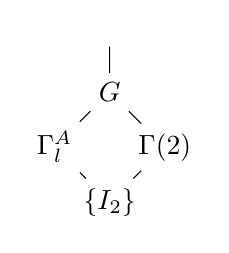
\begin{tikzpicture}[scale=.7]
  \node (sltz) at (0,2) {$\sltz$};
  \node (g) at (0,1) {$G$};
  \node (gl) at (-1,0) {$\Gamma_{l}^A$};
  \node (g2) at (1,0) {$\Gamma(2)$};
  \node (i) at (0,-1) {$\{I_2\}$};
  \draw  (sltz) -- (g) --(gl) -- (i) --(g2) -- (g);  % (a) -- (one) -- (b) -- (zero) -- (c) -- (one) -- (d) -- (zero);
\end{tikzpicture}
\caption{Hasse diagram} \label{fig:hasseDiagram}
\end{figure}

We claim that $\Gamma_{l}^A$ is a non-congruence subgroup if $l$ is not a power of 2.\\ 
Now since $\Gamma(lt) \subset \Gamma(t)$ it suffices to show $ \Gamma(tl) \not\subset \Gamma_l$ for any $t$. We can write $l = 2^q*k$ where $k >1$ odd. From this we can rewrite $ln = 2^q k t = 2^mkn$ with $n$ odd. For the sake of contradiction let us suppose $\Gamma(2^t kn) \subset \Gamma_{l}^A$ for some $m \geq 0$ and odd $n$. \\
The integers $2^m5kn$ and $5kn -4$ are comprime, $2$ is not a common divisor since $5kn -4$ is odd, and also if an odd prime $p \vert 2^m5kn \implies p\vert 5kn$ so it will not divide $5kn -4$. There exists an integer $s$ such that $s(5kn -4) \equiv 1 \mod 2^m5kn$, i.e $s(5kn -4) = 1 + (2^m5kn)h$ for some $h \in \mathbb{Z}$. If we consider this equation modulo 5, we get $s \equiv 1 \mod 5$. Let us write $s = 5r +1$. \\
The matrix $P = B^rABA^{kn-1} =  \left(\begin{array}{ c c } 5 & 2(5kn -4) \\ 2s & \delta \end{array} \right) \in G$ for some $\delta$. Note that the condition on the determinant $\det(P) = 1$ gives $\delta \equiv 1 \mod 2^mkn$, ($\star$). \\
We can also consider the matrix $Q = A^{5kn -4}B^s =  \left(\begin{array}{ c c } \alpha & 2(5kn -4) \\ 2s & 1 \end{array} \right) \in G$ for some $\alpha$. Again the condition on the determinant is $5\delta - 4s(5kn -4) =1$, now consider this modulo $2^m5kn$ and use $(\star)$, to get $5\delta \equiv 5 \mod 2^m5kn$. This implies that $\alpha \equiv 5 \mod 2^m5kn \implies \alpha \equiv 5 \mod 2^mkn$. 

Therefore we can see by considering each entry that $P \equiv Q \mod 2^mkn$. In other words, $PQ^{-1} \in \Gamma(2^mkn)$. But, $E_A(PQ^{-1}) = 1 + (kn-1) + 4 - 5kn = -4kn + 4 \equiv 4 \not \equiv 0 \mod k$.Hence $E_A(PQ^{-1}) \not\equiv 0 \mod l$. This contradicts our assumption that $\Gamma(2^mkn) \subset \Gamma_{l}^A$. Hence, $\Gamma_{l}^A$ cannot be a congruence subgroup.\\
\\
We can determine the index of $\Gamma_{l}^A$. From figure \ref{fig:hasseDiagram} we have, 
$$[\sltz \, : \,\Gamma_{l}^A]= [\sltz \, : \, G][G \, : \, \Gamma_{l}^A] =[\sltz \, : \, G]\cdot \vert \znz[l] \vert = [\sltz \, : \, G]\cdot l$$
Also,
$$ [\sltz \, : \, G] = \frac{[\sltz \, : \, \Gamma(2)]}{[G \, : \, \Gamma(2)]} = \frac{6}{2} =3.$$
So we have $[\sltz \, : \, \Gamma_{l}^A] = 3l$.
\end{example}

\subsection{Local versus index - a criterion}

\begin{theorem} {'Wohlfahrt's criterion'} \label{thm:criterion}\\
Let $G \leq \sltz$ be a subgroup of finite index. Suppose $n$ is a positive integer such that $G \supset \gamma \left(\begin{array}{ c c } 1 & n \\ 0 & 1 \end{array} \right) \gamma^{-1}$ for every $\gamma \in 
\sltz$. Then, $G$ is a congruence subgroup if, and only if, $G \geq \Gamma(n)$. (The notation $G \geq H$ means $H$ is a subgroup of $G$.)
\end{theorem}
\begin{proof}
If $G \geq \Gamma(n)$ then by definition it is a congruence subgroup. \\
For the reverse implication let us assume that $G$ is a congruence subgroup, $G \geq \Gamma(m)$ for some $m$, and that there is a $n$ such that $G \supset \gamma \left(\begin{array}{ c c } 1 & n \\ 0 & 1 \end{array} \right) \gamma^{-1}$ for every $\gamma \in sltz$. (Note in particular $\left(\begin{array}{ c c } 1 & n \\ 0 & 1 \end{array} \right) \in G$).
We wish to show that $G \geq \Gamma(n)$. \\
Let $g = \abcd \in \Gamma(n)$. From the determinant we get $\det(g) = ad -bc = 1 \implies (a,c) =1$ and also since $g \in \Gamma(n)$ we have $n \vert c$ so $(a,nc) =1$. From Lemma \ref{lem:elementaryCoprime} we can find $x \in \mathbb{Z}$ such that $(a + ncx,m) = 1$. Therefore, there exists $y$ such that $y(a + ncx) \equiv 1 \mod m$ $(\star)$. \\
Now let $g_1$ be the product, 
$$g_1 = \left(\begin{array}{ c c } 1 & nx \\ 0 & 1 \end{array} \right)g =  \left(\begin{array}{ c c } a + ncx & b+ndx \\ c & d \end{array} \right) \in \Gamma(n)$$
Moreover from the assumption about $G$, we have for any integer $z$, if we let,
$$g_2 := \left(\begin{array}{ c c } 1 +nz & -n \\ nz^2 & 1-nz \end{array} \right) = \left(\begin{array}{ c c } 1 & 0 \\ z & 1 \end{array} \right) \left(\begin{array}{ c c } 1 & -n \\ 0 & 1 \end{array} \right)\left(\begin{array}{ c c } 1 & 0 \\ -z & 1 \end{array} \right) $$
Then the matrix $g_2$ is in $G$ since it is the inverse of a matrix of the form $\gamma  \left(\begin{array}{ c c } 1 & n \\ 0 & 1 \end{array} \right) \gamma^{-1}$n and $g_2 \in \Gamma(n)$.\\
We have $g_2 g_1 = \left(\begin{array}{ c c } (1+nz)(a+ncx) -nc & \star \\  \star &  \star \end{array} \right)$.\\
If we choose $z = y(c(1-x) + \frac{1-a}{n})$, we get 
\begin{eqnarray*}
(1+nz)(a + ncx) -nc &=& (1 + ny(c(1-x) + \frac{1-a}{n})(a + ncx) - nc \\
&=& a+ncx + ny(a+ncx)(c(1-x) + \frac{1-a}{n} \\
\text{ use } (\star) &=& a + ncx + n(1 +mt)(c(1-x) + \frac{1-a}{n} \text{ for some } t \in \mathbb{Z} \\
&=& a + ncx + nc - ncx + 1 -a + nmt(c(1-x)) + mt(1-a) \\
& = & 1 + (1-a)mt + nmt(c(1-x)) \\
(a \equiv 1 \mod n) & \equiv & 1 \mod mn  
\end{eqnarray*}
Let
$$h = \left(\begin{array}{ c c } 1 +nz & -n \\ nz^2 & 1-nz \end{array} \right) = \left(\begin{array}{ c c } 1 & 0 \\ z & 1 \end{array} \right) \left(\begin{array}{ c c } 1 & -n \\ 0 & 1 \end{array} \right)\left(\begin{array}{ c c } 1 & 0 \\ -z & 1 \end{array} \right)\left(\begin{array}{ c c } 1 & nx \\ 0 & 1 \end{array} \right),\quad  z = y(c(1-x) + \frac{1-a}{n}).$$
Then by inspection we see $h \in G \cap \Gamma(N)$. Now consider $hg \in \Gamma(n)$.\\
The matrix $hg$ can be written in the form $\left(\begin{array}{ c c } \star & nu \\ nv & \star \end{array} \right)$ since $hg \in \Gamma(n)$.\\
From the work above we also have $hg \equiv \left(\begin{array}{ c c } 1 & \star \\ \star & \star \end{array} \right) \mod mn$. So we combine these to get $ hg  \equiv \gamma = \left(\begin{array}{ c c } 1 & nu \\ nv & \star \end{array} \right) \mod mn$.\\
The condition on the determinant gives $\gamma \equiv  \left(\begin{array}{ c c } 1 & nu \\ nv & 1 + n^2uv \end{array} \right) \mod mn$.
We may decompose this as 
\begin{align*}
\gamma &\equiv  \left(\begin{array}{ c c } 1 & 0 \\ nv & 1 \end{array} \right) \left(\begin{array}{ c c } 1 & nu \\ 0 & 1 \end{array} \right) \\
&\equiv \left(\begin{array}{ c c } 0 & 1 \\ v & 0 \end{array} \right) \left(\begin{array}{ c c } 1 & n \\ 0 & 1 \end{array} \right) {\left(\begin{array}{ c c } 0 & 1 \\ v & 0 \end{array} \right)}^{-1} \left(\begin{array}{ c c } u & 0 \\ 0 & 1 \end{array} \right)^{-1}\left(\begin{array}{ c c } 1 & n \\ 0 & 1 \end{array} \right) \left(\begin{array}{ c c } u & 0 \\ 0 & 1 \end{array} \right)
\end{align*}
So if consider $\gamma' =  \left(\begin{array}{ c c } 1 & nu \\ nv & 1 + n^2uv \end{array} \right) \equiv \gamma$ be an element in $\sltz$, then $\gamma' \in G$.\\
\\
We use, $\gamma^{-1}hg \equiv I_2 \mod mn$, to say $\gamma'^{-1}hg \in \Gamma(mn) \leq \Gamma(m) \leq G$. Finally since $\gamma',g \in G$ we can conclude $g \in G$ and so $\Gamma(n) \leq G$.
\end{proof}

\begin{example}
We can use the above criterion to obtain another example of a non-congruence subgroup. \\
Let us recall the homomorphism $E_A \, : \, w(A,B) \rightarrow \mathbb{Z}$ from Example \ref{ex:noncongruenceEA}, and define $E_B \, : \, w(A,B) \rightarrow \mathbb{Z}$ similarly, as the sum of the exponents of $B$ occurring in a word $w$. From these we can define a new homorphism, $E_{A,B} \, : \, w(A,B) \rightarrow \mathbb{Z} \times \mathbb{Z}$, where $E_{A,B}(w) = (E_A(w), E_B(w))$.\\ 
For a positive integer $l$ let us define 
\begin{eqnarray*}
\Gamma_{l}^{A,B} &=& \{g \in w(A,B) \, :\, E_A(g) \equiv E_B(g) \equiv 0 \mod l\} \\
\ker(w(A,B) & \rightarrow & \mathbb{Z} \times \mathbb{Z} \rightarrow \znz[l] \times \znz[l]
\end{eqnarray*} This group is a subgroup of the non-congruence subgroup, $\Gamma_{l}^A$ from example \ref{ex:noncongruenceEA}.\\

We claim: If $l$ is not a power of 2. then $\Gamma_l$ is not a congruence subgroup. \\
If it were a congruence subgroup, then $\Gamma_p \geq \Gamma_l$ would also be a congruence subgroup for any odd prime divisor $p$ of $l$.

Consider the matrix, $A^{2p} = \left(\begin{array}{ c c } 1 & 2p \\ 0 & 1 \end{array} \right) \in \Gamma_p$, then for any $\gamma \in \sltz$ we have $E_A(\gamma A^p \gamma^{-1}) = E_A(\gamma) + E_A(A^p)+ E_A(\gamma^{-1}) = E_A(\gamma) + E_A(A^p) - E_A(\gamma) = E_A(A^p) = p \equiv 0 \mod p$, and similarly $E_B(\gamma A^p \gamma^{-1}) = E_B(\gamma A^p) = 0 \equiv 0 \mod p$. So $\gamma A^p \gamma^{-1} \in \Gamma_p$ and the criterion in Theorem \ref{thm:criterion}, is satisfied for $n = 2p$, thus $ \Gamma_p \geq \Gamma(2p)$.
\\
Thus the index $[\sltz \, : \, \Gamma_p]$ divides $[\sltz \,: \, \Gamma(2p)]$. We will see that this gives a contradiction.
\\

We obtained an expression for index's of congruence subgroups in Corollary \ref{cor:indexListChain},
 $$[\sltz \,: \, \Gamma(2p)] = (2p)^3\prod_{p \mid 2p}(1 - 1/p^2) = 8p^3( 1 - 1/4)(1 - 1/p^2) = 6p(p^2 -1)$$
\\
From the presentation of $\Gamma_p$ as a kernel, we get that the index $[w(A,B) \, : \, \Gamma_p] = \vert \znz[p] \times \znz[p] \vert = p^2$. We computed in Example \ref{ex:noncongruenceEA}, that $[\sltz \, : \, w(A,B)] = 3$ so we can combine these two to get $[\sltz \, : \, \Gamma_p] = 3p^2$. 
\\
Suppose then that $[\sltz \, : \, \Gamma_p] \vert [\sltz \,: \, \Gamma(2p)]$, then $$3p^2 \vert 6p(p^2 -1) \implies p \vert 2(p^2 -1) \stackrel{\text{p odd}}{\implies} p \vert (p^2 -1) $$

This is a contradiction so $\Gamma_l$ cannot be a congruence subgroup if it contains an odd prime factor.
\end{example}

\section{Conclusion}
For another construction of non-congruence subgroups see \citep{hsu1996identifying}, in this a method, based on permutation representations of $\psltz$, of identifying congruence subgroups is detailed.\\
The question of determining whether or not finite-index subgroup of $\sltz$ that are not congruence subgroups exist, is more generally known as the Congruence Subgroup Problem. We have shown they do exist for $\sltz$ but it is easy to pose the problem similarly for $SL_n(\mathbb{Z})$. It was actually shown in \citep{bass1964} that for $n > 2$ every finite index subgroup of $SL_n(\mathbb{Z})$ are congruence subgroups. \\
Even further it is possible to define the notion of congruence for more general number fields $K$, a more general result about $SL_n(\mathcal{O}_K$ is proven in \citep{bassSolution}.\\
\\
Python code written for this project is available at https://github.com/MarcoForte/UndergradThesis
The code includes, the generating of the images, and implementations of algorithms like those described geometric and algebraic proof that $\langle S, T \rangle = \sltz$.